\documentclass{article}
\usepackage[utf8]{inputenc}

\title{SRS - Product Perspective}
\author{Nardus van der Vyver }
\date{February 2017}

\usepackage{natbib}
\usepackage{graphicx}

\begin{document}

\maketitle

\section{System Interfaces}
The System Interface is basically all the internal interfaces between the application (software) and everything else within the bigger system.
The System Interface includes all the interfaces and their functionality to accomplish the system requirement, interfaces include user (screen), hardware (mobile device), software (NavUP) and communications (Wi-Fi) � interfaces.

\section{User Interfaces}
The User Interfaces include:
The NavUP application with all its interactive parts (Buttons, scroll bars, search bars, links etc.)
The NavUP application in the form of how it is embodied on the screen.
The keyboard used in-app to type a destination or so on.
The touch screen used in order to navigate the application effectively.\\
*The User Interface entails accepting input via devices like the touch screen or keyboard in order to provide output in the form of a Graphical User Interface on the portable device of choice. The GUI (Graphical User Interface) provides the output that will guide the user on his/her journey through campus. 

\section{Hardware Interfaces}
The Hardware Interfaces include:
The mobile device of choice (Phone/Tablet).
*not taking pc or laptops into consideration because of the mobile nature of the app.
Hardware like the screen (used to display the user interface of the application and record user actions like typing and selecting).
The mobile devices� network receiver used to connect to campus Wi-Fi.
The accelerometer of the phone that can be used to measure how fast or where the person is walking while in-app.
The devices memory(primary and secondary)\\
*The Hardware Interface is one of the core parts of the project (The input/output device), as the software product (NavUP) has to connect with the hardware components of the device. 

\section{Software Interfaces}
The Software Interfaces include:
The Mobile device OS (Operating System), that will handle all the requests made by the NavUP application.
The NavUP application that will run on the phone.\\
*The Software Interfaces will provide access to the mobile devices resources like the storage (saving locations in-app), CPU(processing any requests needed).

\section{Communications Interfaces}
The Communications Interfaces include:
The mobile devices� network receiver (to connect to Wi-Fi) and program used to translate the signals received. 
The Wi-Fi sign on the mobile device that will give indication of signal strength and connectivity.\\
*The Communications Interface handles requests to and from the Wi-Fi and application server that will give the user the experience and output needed.


\begin{figure}[h!]
\centering
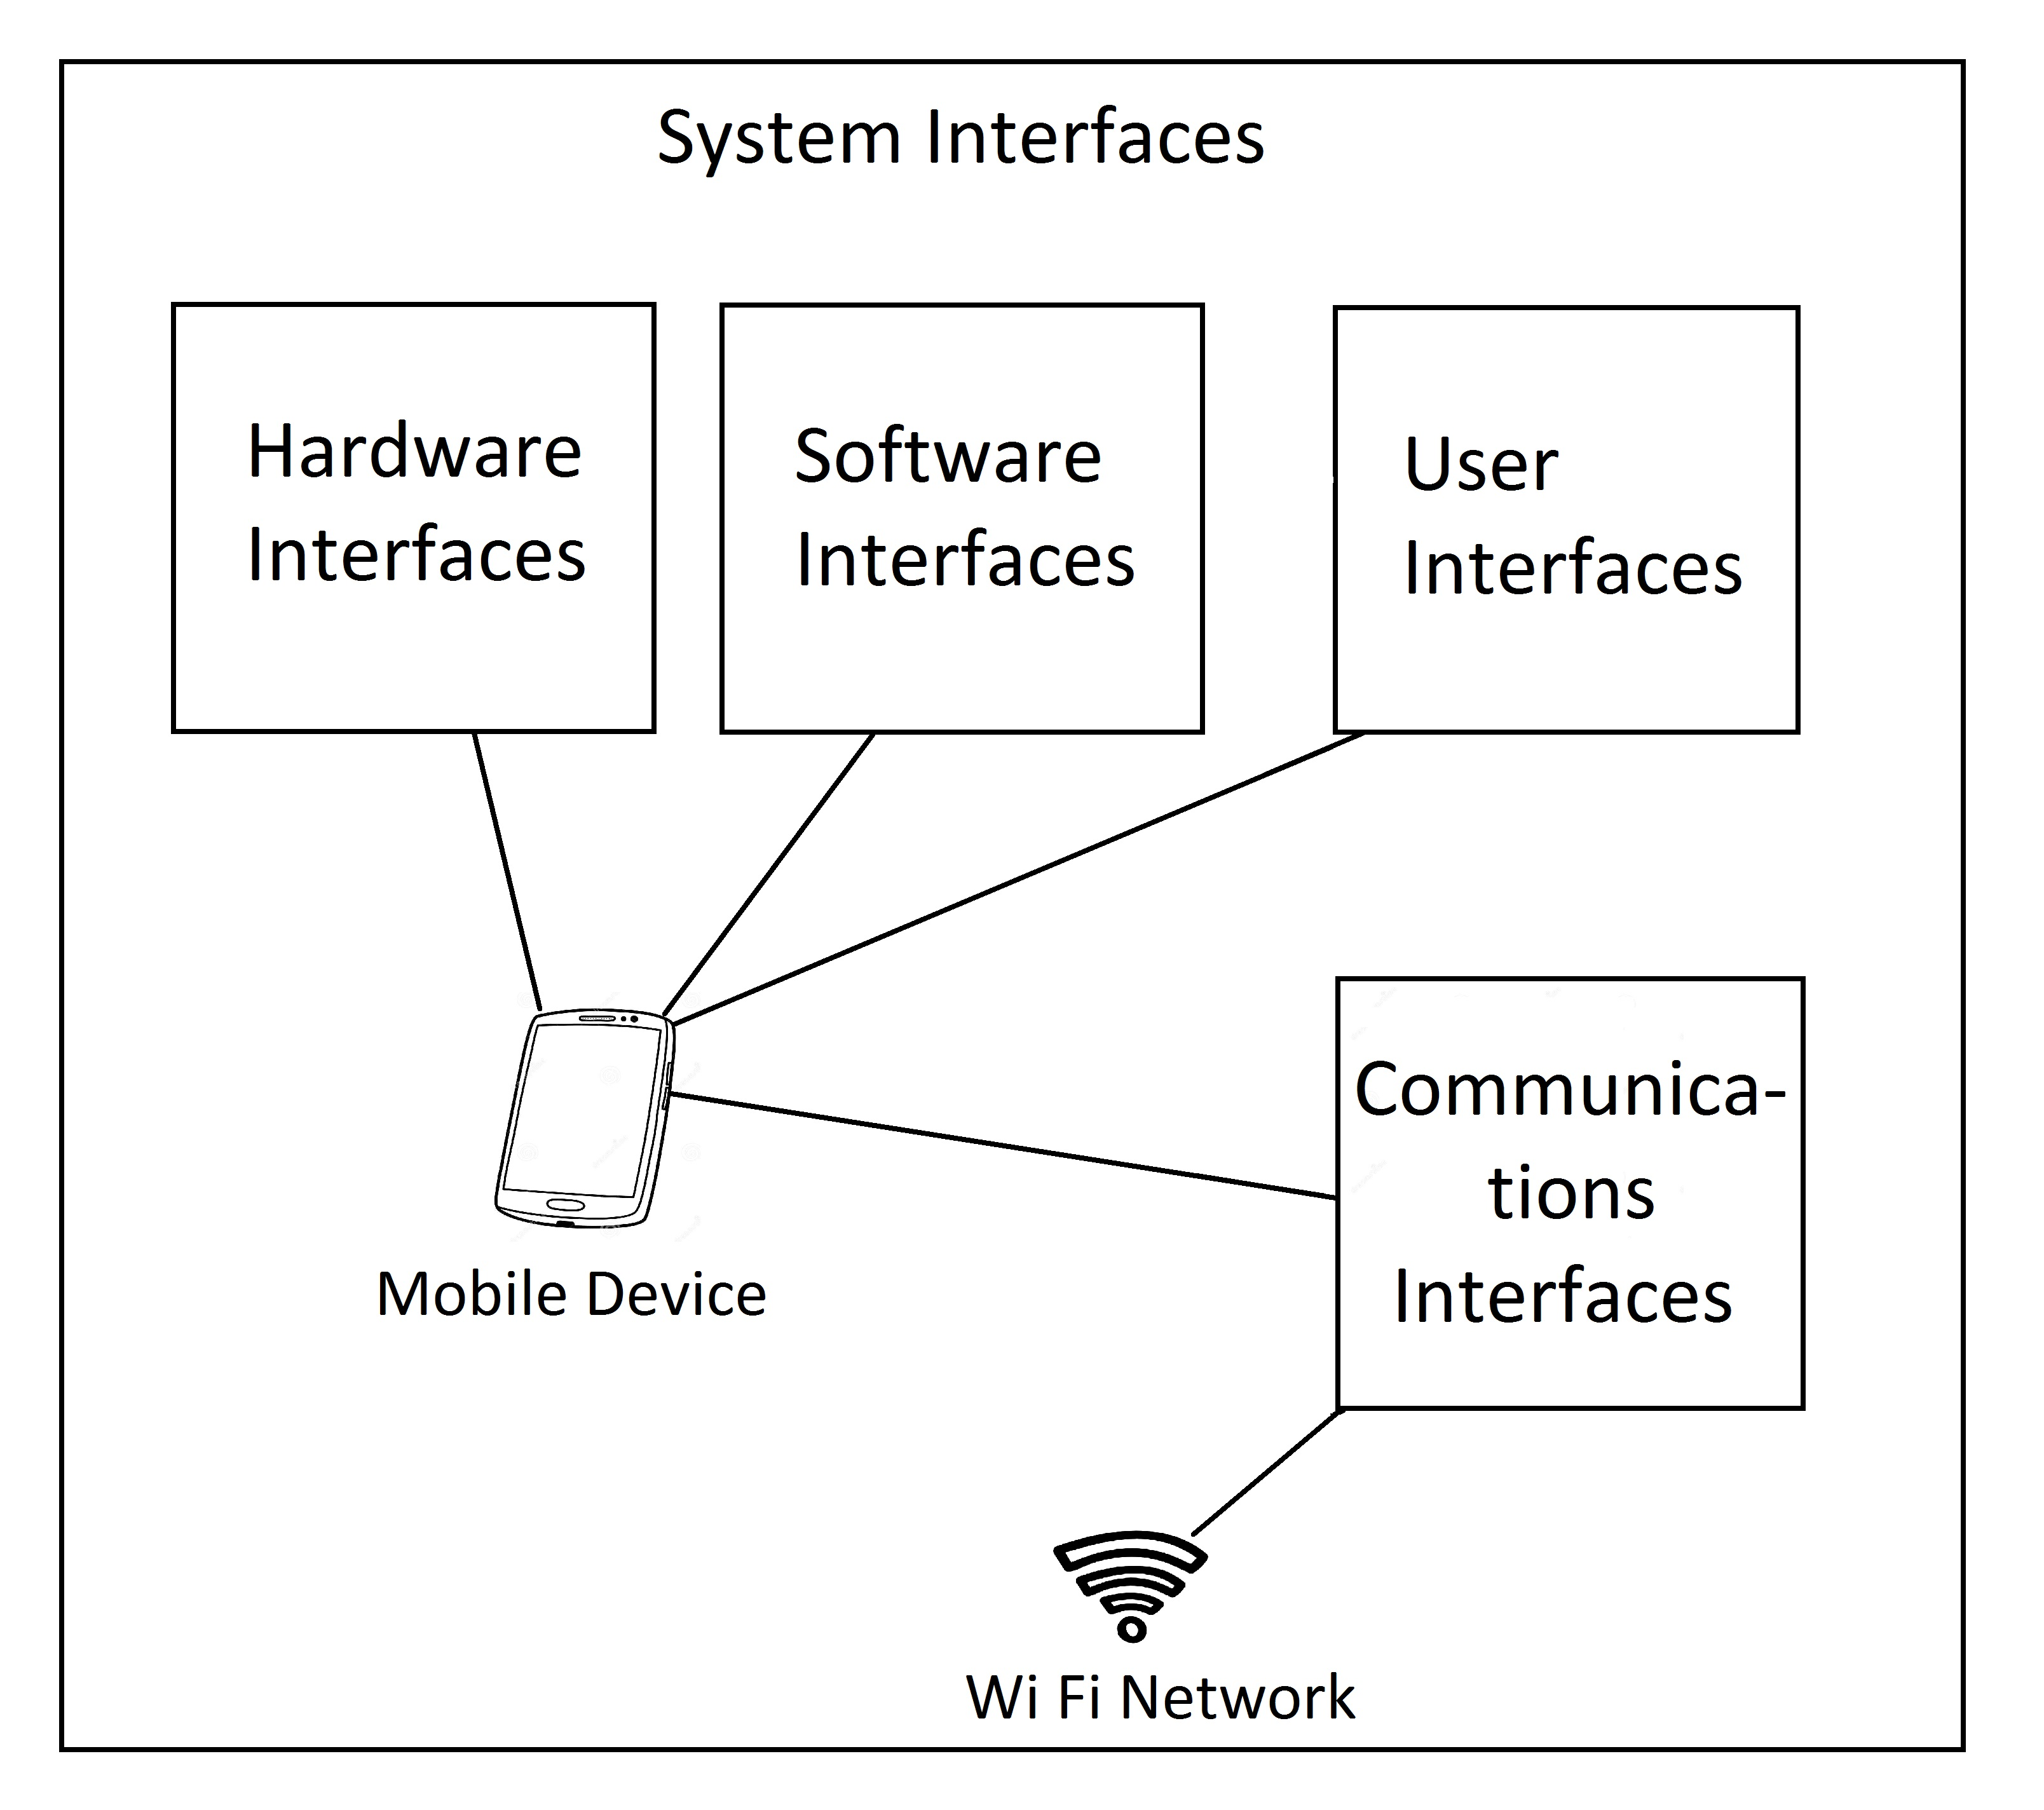
\includegraphics[scale=0.1]{BLockDiagram.jpg}
\caption{Block Diagram}
\label{fig:block diagram}
\end{figure}

\section{Memory}
\textbf{Primary Memory:}
The primary memory refers to the RAM (Random Access Memory) of the mobile device. 
The RAM is used to store information intended for immediate use within the app. 
A limit that primary storage brings is that it is volatile, so no in-app data can be stored and retrieved later.
Another limit is that RAM can vary in size, the bigger the size the better the app will perform (because more information can be stored and accessed quickly), but that is dependent on the various different mobile devices.\\
\textbf{Secondary Memory:}
The secondary memory includes the devices internal hard drive as well as external SD cards.
Secondary memory is where the program as well as the saved data (locations and other in-app details) is kept and stored on a long term basis. 
A limit of secondary storage is that it is much slower that primary memory and may cause the application to take a while to open.
Another limit is that the data stored can be gone if stored on SD card and the card is removed.
If the mobile device is broken or destroyed you will not be able to access your saved data and information.


\end{document}
